\documentclass{beamer}
\usepackage[utf8]{inputenc}
%\usepackage[latin1]{inputenc}
%\usepackage[cyr]{aeguill}
\usepackage[T1]{fontenc}
\usepackage{graphicx}
\usepackage{amsmath,amsfonts,amsthm,amssymb}
\usepackage{algorithm}
\usepackage{algorithmic}
\usepackage{cases}
%\usepackage[]{algorithm2e}
\usepackage{hyperref}
\usepackage{color}
\usepackage{pstricks}
%\usepackage{stmaryrd}
%\usepackage{enumitem} 
\usepackage{bm,bbm}
\usepackage{array}
\usepackage{relsize,exscale}
\usepackage{caption}
\usepackage{subcaption}
%\usepackage{tikz}
%\usetikzlibrary{calc}
\DeclareMathOperator*{\argmin}{argmin}
\definecolor{ao(english)}{rgb}{0.0, 0.5, 0.0}
\definecolor{armygreen}{rgb}{0.29, 0.33, 0.13}
\definecolor{britishracinggreen}{rgb}{0.0, 0.26, 0.15}
\definecolor{cadmiumgreen}{rgb}{0.0, 0.42, 0.24}
\definecolor{indigo}{rgb}{0.29, 0.0, 0.51}
\definecolor{lightgray}{gray}{0.85}
\definecolor{midnightblue}{rgb}{0.1, 0.1, 0.44}
\definecolor{burntorange}{rgb}{0.8, 0.33, 0.0}
\definecolor{royalblue}{rgb}{0.25, 0.41, 0.88}
\definecolor{darkmagenta}{rgb}{0.55, 0.0, 0.55}
\definecolor{byzantine}{rgb}{0.74, 0.2, 0.64}
\definecolor{blue-violet}{rgb}{0.54, 0.17, 0.89}
\definecolor{brown-traditional}{rgb}{0.59, 0.29, 0.0}
\definecolor{brown-web}{rgb}{0.65, 0.16, 0.16}
\definecolor{burgundy}{rgb}{0.5, 0.0, 0.13}
\definecolor{electricpurple}{rgb}{0.75, 0.0, 1.0}
\definecolor{gray}{rgb}{0.5, 0.5, 0.5}
\definecolor{goldenbrown}{rgb}{0.6, 0.4, 0.08}
\definecolor{armygreen}{rgb}{0.29, 0.33, 0.13}
\definecolor{calpolypomonagreen}{rgb}{0.12, 0.3, 0.17}
\definecolor{caputmortuum}{rgb}{0.35, 0.15, 0.13}
\definecolor{carmine}{rgb}{0.59, 0.0, 0.09}
\definecolor{chocolate-traditional}{rgb}{0.48, 0.25, 0.0}
\definecolor{lincolngreen}{rgb}{0.11, 0.35, 0.02}
\definecolor{magenta}{rgb}{1.0, 0.0, 1.0}
\definecolor{auburn}{rgb}{0.43, 0.21, 0.1}
\definecolor{bole}{rgb}{0.47, 0.27, 0.23}
\definecolor{bulgarianrose}{rgb}{0.28, 0.02, 0.03}
%\usepackage[dvipsnames]{xcolor}
%\xdefinecolor{vert_olive}{named}{OliveGreen}
%\xdefinecolor{bleuviolet}{named}{BlueViolet}
%\xdefinecolor{bleucadet}{named}{CadetBlue}
%\xdefinecolor{bleunuit}{named}{MidnightBlue}
\graphicspath{{./Figures/}}

\renewcommand{\div}{\mathrm{div}}
\usepackage{graphicx} 
%\usepackage{epstopdf}

\usetheme{Frankfurt}

\title[WCCM 2018]{Adaptive inexact semismooth Newton methods for the contact problem between two membranes}
\author[Jad Dabaghi]{\underline{Jad Dabaghi}, Vincent Martin, Martin Vohral\'ik}
\institute[]{Inria Paris \& Université Paris-Est}
\date{WCCM, New-York, July 23 2018}
\subject{Numerical Analysis}
\input{paper_commands.tex}

\setbeamertemplate{navigation symbols}{}
\setbeamercovered{transparent}
%\AtBeginSection[] {
%     \begin{frame}<beamer>[noframenumbering]
%         \frametitle{Outline}
%         \tableofcontents[currentsection]
%     \end{frame}
%}
%

\setbeamersize{text margin left=0.2 cm}
\setbeamersize{text margin right= 0.3 cm}
\setbeamersize{sidebar width left=0 cm}
\setbeamersize{sidebar width right= 0 cm}



\begin{document}

% \section{Introduction}
% \subsection{Introduction}

\begin{frame}
\maketitle
\includegraphics[scale=0.3]{INRIA-SCIENTIFIQUE-UK-RVB}
\hfill \includegraphics[scale=0.08]{Logo_ponts_paristech}

\end{frame}

%\begin{frame}
%\frametitle{Adaptive inexact semi smooth Newton methods for a contact between two membranes.}
%\includegraphics[scale=0.2]{inria}
%\hspace{5 cm}
%\includegraphics[scale=0.2]{upmc}
%\vspace{0.6 cm}
%\fbox{
%\begin{minipage}{1\textwidth}
%     \begin{center}
%           Pierre and Marie Curie University/INRIA Paris SERENA team
%     \end{center}
%\end{minipage}}
%\vspace{0.2 cm}
%\begin{center}
%Jad Dabaghi
%\end{center}
%\underline{Supervisors}: 
%\begin{itemize}
%\item  Martin Vohralik
%\item  Vincent Martin
%\end{itemize}
%\vspace{-0.6 cm}
%\hspace{8 cm}
%\textcolor{blue}{April 19 2017}
%\end{frame}
%


\begin{frame}<beamer>[noframenumbering]
     \frametitle{Outline}
     \tableofcontents
\end{frame}







\setcounter{tocdepth}{4}
\section{Introduction}
\subsection{}
\begin{frame}[t]
\defbeamertemplate*{footline}{infolines theme frame plus slide}{\setcounter{slidenumber}{\insertpagenumber}\addcounter{slidenumber}{-\insertframestartpage}\addcounter{slidenumber}{1}}
%\title{Introduction}
\frametitle{Introduction}
\vspace*{-0.3 cm}
\textcolor{red}{\textbf{System of variational inequalities:}}\\
\vspace*{0.2 cm}
Find $u_1$, $u_2$, $\lambda$ such that
\begin{equation*}
\dps
\left\lbrace\begin{array}{llccc}
\dps -\mu_1 \Delta u_1-\lambda = f_1 \qquad \mbox{in} \quad \Omega, \\
\dps -\mu_2 \Delta u_2+\lambda = f_2 \qquad \mbox{in} \quad \Omega,\\
\dps (\textcolor{electricpurple}{u_1-u_2})\textcolor{carmine}{\lambda}=0, \quad \textcolor{electricpurple}{u_1-u_2 \geq 0}, \quad 
\textcolor{carmine}{\lambda \geq 0} \qquad \mbox{in} \quad \Omega, \hspace{0.2 cm}\\
\dps u_1=g > 0 \qquad \mbox{on} \quad\partial \Omega,\\
\dps u_2=0 \qquad \mbox{on} \quad\partial \Omega.
\end{array}
\right.
%\label{eq:modele_initial_membrane}
\end{equation*}
\vspace{-0.7cm}
\begin{figure}[t]
\begin{subfigure}[normal]{0.46\textwidth} 
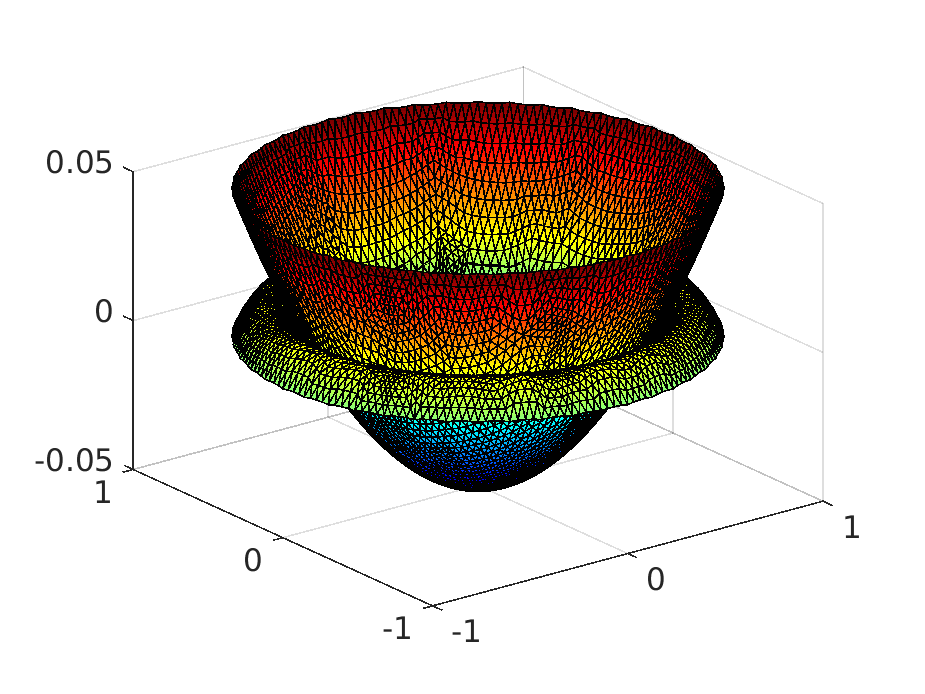
\includegraphics[width=\textwidth]{fig_article/fig_membrane_cv.eps}    
\label{ref:position_membrane_convergence}
\end{subfigure}
\qquad
\begin{subfigure}[normal]{0.46\textwidth}
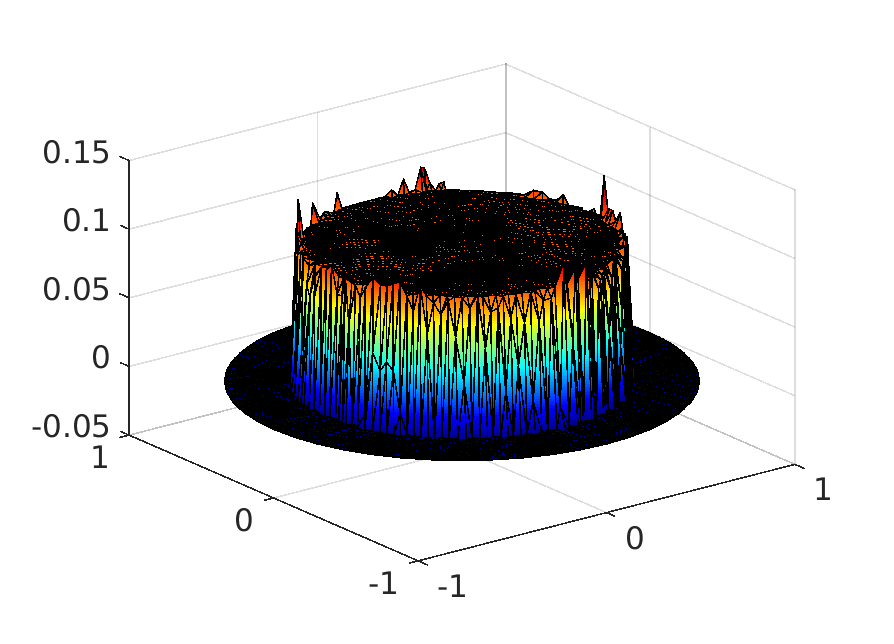
\includegraphics[width=\textwidth]{fig_article/fig_lambda_cv.eps}     
\label{ref:lambda_membrane_convergence} 
\end{subfigure}
\end{figure}
\vspace*{-4cm}\hspace*{0.95cm}$u_1$\\
\vspace*{0.7cm}\hspace*{0.85cm}$u_2$
\end{frame}
%\begin{frame}
%\frametitle{Introduction}
%\textbf{\textcolor{red}{Motivation}}
%\begin{itemize}
%\item
%Finite element discretization: 
%$\mathcal{A}(\Xh) = \bF$. 
%\item 
%Resolution via inexact \textbf{semi smooth} Newton method 
%%s$\mathbb{A}^{k-1}\Xhki + \Rhki = \bF^{\textcolor{blue}{k}-1}$
%\item
%A posteriori error estimate: 
%$\dps |||\bu-\uhki||| \leq \left\{\sum_{K \in\Th}\eta_K^2(\uhki)\right\}^{\frac{1}{2}}$.
%\item Adaptive inexact resolution and  adaptive stopping criteria.
%\item Numerica experiments to confirm the strength of our method.
%\end{itemize}
%\footnotesize
%\begin{thebibliography}{10}
%\bibitem{VorErn:2013}
%Alexandre Ern and Martin Vohral{\'{\i}}k.
%\newblock Adaptive inexact {N}ewton methods with a posteriori stopping criteria
%  for nonlinear diffusion {PDE}s. {\em SIAM J. Sci. Comput.}, 35(4):A1761--A1791, 2013.
%\end{thebibliography}
%\end{frame}
\begin{frame}
\section{Model problem and its discretization}
\subsection{}  
\frametitle{Continuous model problem and setting}
\begin{itemize}
\item $H_g^1(\Omega)\hspace{-0.1 cm} =\hspace{-0.1 cm} \left\{u\in H^1(\Omega), \hspace{0.1 cm} u=g \hspace{0.1 cm} \mbox{on} \hspace{0.1 cm} \partial \Omega\right\}$ \quad $\Lambda=\left\{\chi\in L^2(\Omega), \: \textcolor{carmine}{\chi \geq 0} \: \mbox{on} \hspace{0.1 cm} \Omega\right\}$
\item
$\Kg= \left\{(v_1,v_2)\in H_g^1(\Omega)\times H_0^1(\Omega),\: \textcolor{electricpurple}{v_1-v_2 \geq 0} \; \; \mbox{on} 
\hspace{0.1 cm} \Omega \right\}$
\end{itemize}
\textbf{Weak formulation:}
For $(f_1,f_2)\in L^2(\Omega)\times L^2 (\Omega)$ and $g > 0$ find $(u_1,u_2,\lambda)\in H_g^1(\Omega)\times H_0^1(\Omega) \times \Lambda$ such that
\begin{equation*}
\left\lbrace\begin{array}{llccc}
\dps \sum_{\ialf=1}^2 \mu_i \left(\nab u_i,\nab v_i\right)_{\Omega} - \left(\lambda,v_1-v_2\right)_{\Omega} = \sum_{\ialf=1}^2\left(f_i,v_i\right)_{\Omega} \quad \forall (v_1,v_2) \in \left(H_0^1(\Omega)\right)^2 \\
\left(\chi - \lambda,u_1-u_2\right)_{\Omega} \geq 0 
\quad \forall \chi \in \Lambda.
\end{array}
\right.
\end{equation*}
\hspace{4.5 cm}\textcolor{cadmiumgreen}{\textbf{equivalent to}}\\
\textbf{Reduced problem:}
\begin{equation*}
\dps \sum_{\ialf=1}^2 \mu_i \left(\nab u_i,\nab \left(v_i-u_i\right)\right)_{\Omega} \geq \sum_{\ialf=1}^2\left(f_i,v_i-u_i\right)_{\Omega} \quad \forall \bv = (v_1,v_2)\in ~\Kg.
\end{equation*}

\textcolor{red}{\textbf{Existence and uniqueness based on Lions-Stamppachia Theorem}} (Ben Belgacem \eal \ 2008)
% \tiny
% \begin{thebibliography}{10}
%   \bibitem{VorBer:2008}
% Faker Ben~Belgacem, Christine Bernardi, Adel Blouza, and Martin
%   Vohral{\'{\i}}k.
% \newblock A finite element discretization of the contact between two membranes.
% \newblock {\em M2AN Math. Model. Numer. Anal.}, 43(1):33--52, 2008.
% \end{thebibliography}
\end{frame}
%%
\begin{frame}
\frametitle{Discretization by finite elements}
\textbf{Notation:} 
%Let $\Th$ be a conforming mesh of $\Omega$ in the sens of Ciarlet. 
$\Th$: conforming mesh, $\Vdp$: set of DOFs, $\Ndp$ number of DOFs, $\Vh$: set of vertices\\
%\item 
%$\Vh$: vertices of $\Th$, $\Vhint$: interior vertices, $\Vhext$: exterior vertices. 
%\item 
%$\omega_\ba$: patch of elements of $\Th$ that share $\ba$ and ${\bf n}_{\omega_{h}^{\ba}}$ its outward unit normal.
%\item  
%$\psi_{h,\ba}$: Lagrange basis functions,
%$N_{h,\ba}$: Nnumber of elements forming a support of the basis functions
%\item
%$N_{h,\ba}$: Nnumber of elements forming a support of the basis functions, $\ba \in \Vhint$
%\item
%$h_K$: diameter of a triangle $K$.\quad $h=\max h_K$, $M_{\ba} = \left(\psi_{h,{\ba}},1\right)_{\omega_{\ba}} > 0$ 
\vspace{0.2 cm}
\textcolor{cadmiumgreen}{\textbf{Spaces for the discretization:}}\\
$\Xghp=\left\{v_h \in \mathcal{C}^0(\overline{\Omega}),  {v_h}_{|K} \in \Pp (K), \ \forall K \in {\mathcal{T}}_h, \hspace{0.2 cm} v_h=g \hspace{0.2 cm} \mbox{on} \hspace{0.2 cm} \partial \Omega\right\}$\\
\vspace*{0.3 cm}
$\Xzerohp =\left\{v_h \in \calC^0(\overline{\Omega}); \ {v_h}|_{K} \in \Pp (K), \quad \forall K \in \Th \right\} \cap H_0^1(\Omega)$
\\
\vspace*{0.3 cm}
$\dps \Kghp=\left\{(\vunh,\vdeuxh) \in \Xghp \times \Xzerohp, \ \textcolor{electricpurple}{\vunh(\xl)-\vdeuxh(\xl)} \geq 0 \ \ \forall \xl \in \Vdp \right\} \textcolor{red}{\not \subset \Kg}$\\
\vspace*{0.2 cm}
\textcolor{cadmiumgreen}{\textbf{Discrete reduced problem:}} find $\dps \uh=(\uunh,\udeuxh) \in \Kghp$ such that
\begin{equation*}
\dps \sum_{\ialf=1}^2 \mu_i \left(\nab u_{ih},\nab \left(v_{ih}-u_{ih}\right)\right)_{\Omega} \geq \sum_{\ialf=1}^2\left(f_i,v_{ih}-u_{ih}\right)_{\Omega} \quad \forall \bv_h = (v_{1h},v_{2h})\in ~\Kg.
\end{equation*}
\textcolor{midnightblue}{\textbf{Resolution techniques:}}
 Projected Newton methods (Bertsekas 1982), Active set Newton method (Kanzow 1999), Primal-dual active set strategy (Hinterm\"uller 2002). 
\vspace{0.5 cm}
\end{frame}
\begin{frame}
\textcolor{cadmiumgreen}{\textbf{Characterization of the discrete lagrange multiplier:}}
\begin{equation*}
\left\lbrace\begin{array}{rclcc}
\dps \left\langle \lambih,v_{1h}\right\rangle _h&=& \hspace{0.8em}
\dps \mu_1 \left(\nab \uunh, \nab v_{1h}\right)_{\Omega} - \left(f_1, v_{1h}\right)_{\Omega} \quad &\forall v_{1h} \in \Xzerohp,\\
\dps \left\langle \lambiih,v_{2h}\right\rangle _h&=& \dps
-\mu_2 \left(\nab \udeuxh, \nab v_{2h}\right)_{\Omega} + \left(f_2, v_{2h}\right)_{\Omega} \quad &\forall v_{2h} \in \Xzerohp,
\end{array}
\right. 
\end{equation*}
where $\forall \left(w_h ,v_h\right) \in \Xzerohp \times \Xzerohp$
\begin{numcases}
{\left\langle w_h ,v_h \right\rangle_h =}
\dps \sum_{\ba \in \Vhint} w_h(\ba) v_h(\ba) \left(\psiha,1\right)_{\Omega}  \quad &\mbox{if} \quad p=1, 
\\ 
\nonumber \dps \left(w_h, v_h\right)_{\Omega} \quad &\mbox{if} \quad p $\geq$ 2  
\end{numcases}
\begin{lemma}
\begin{itemize}
\item
The functions $\lambih$ and $\lambiih$ coincide. We set $\lambda_h=\lambih=\lambiih$.
\item
$\left\langle \lambh ,\psihl \right\rangle_h \geq 0.$
\end{itemize}
\end{lemma}
\begin{definition}
\begin{equation*}
\Lahp = \left\{v_h \in \Xzerohp; \ \left\langle v_h ,\psihl \right\rangle_h \geq 0 \quad \forall \left(\psihl\right)_{1 \leq l \leq \Ndp} \in \Xzerohp \right\}. %\ \not \subset \ \Lambda
\end{equation*}
\end{definition}
\end{frame}
\begin{frame}
\frametitle{Application to $\Pone$ finite elements}
\textcolor{cadmiumgreen}{\textbf{Conforming spaces}}
\begin{itemize}
\item
$\dps \Kghone=\left\{(\vunh,\vdeuxh) \in \Xghone \times \Xzerohone, \ \textcolor{electricpurple}{\vunh(\ba)-\vdeuxh(\ba)} \geq 0 \ \ \forall \ba \in \Vh \right\} \textcolor{red}{\subset \Kg}$\\
\item
$\Lahone = \left\{v_h \in \Xzerohone; \ \textcolor{carmine}{v_h({\ba}) \geq 0}  \quad \forall \ba \in \Vhint \right\} \ \textcolor{red}{\subset \Lambda}$
\end{itemize}
\vspace{0.5 cm}
\textcolor{cadmiumgreen}{\textbf{Weak formulation}} (Ben Belgacem \eal \ 2008)  \\
find $(\uunh,\udeuxh,\lambh)\in \Xghone \times \Xzerohone \times
\Lahone$ s.t  $\forall(\vunh,\vdeuxh,\chi_h) \in \Xzerohone \times \Xzerohone
\times \Lahone$
\begin{equation*}
\begin{array}{lcl}
\dps \sum_{\ialf=1}^2 \mu_\ialf \left(\nab u_{\ialf h}, \nab v_{\ialf h}\right)_{\Omega} 
- \hspace{-0.2 cm}\sum_{\ba\in \Vhint} \hspace{-0.15 cm} \lambh(\ba)(\vunh-\vdeuxh)(\ba) \left(\psiha,1\right)_{\Omega}
=  \dps \sum_{\ialf=1}^2 \left(f_\ialf,v_{\ialf h}\right)_{\Omega}, \\
\dps \textcolor{electricpurple}{(u_{1h}-u_{2h})(\ba) \geq 0}, \: \textcolor{carmine}{\lambda_h(\ba) \geq 0}, \: \textcolor{carmine}{\lambda_h(\ba)} \textcolor{electricpurple}{(u_{1h}-u_{2h})(\ba)}=0.
\end{array}
\end{equation*}
\alert{\hspace{2 cm}\textbf{Can we reformulate the discrete constraints?}}
\end{frame}
\begin{frame}
\frametitle{Discrete complementarity problem}
\begin{definition}
A function $f: {{\R}^n \times \R^n} \rightarrow \R^n$ is a C-function if
\begin{equation*}
\forall(\ba,\bb)\in {\R}^n \times \R^n \quad f(\ba,\bb)=0 \quad \iff \quad
\ba \geq0, \quad \bb \geq0, \quad \ba \bb=0.
\end{equation*}
\end{definition}
For any C-function ${\bf C}$, the discretization reads 
\begin{equation*}
\left\lbrace\begin{array}{llccc}
 \mathbb{E}\Xh &= \bF\\
{\bf C}(\X_h)&=0.
\end{array}
\right.
\quad \mbox{\textcolor{red}{\textbf{$\bf C$ is not Fréchet differentiable!}}}
\end{equation*}
\textcolor{cadmiumgreen}{\textbf{ Example: semismooth "min" function}} 
\begin{equation*}
\CFun(\bXunh-\bXdeuxh,\bXtroish) =\min \left(\bXunh-\bXdeuxh, \bXtroish\right)
\end{equation*}
\textcolor{cadmiumgreen}{\textbf{Example: semismooth "Fischer-Burmeister" function}}
\begin{equation*}
\CFun(\bXunh-\bXdeuxh,\bXtroish)=\sqrt{\left(\bXunh-\bXdeuxh\right)^2 + \bXtroish^2} - (\bXunh-\bXdeuxh + \bXtroish)
\end{equation*}
The vector of unknowns has the following block structure
\begin{equation*}
\Xh^{T}=
\left(\bXunh, \bXdeuxh, \bXtroish\right)^{T} \in \mathbb{R}^{3 \Nh}
\end{equation*}
\end{frame}
\section{Semismooth Newton method}
\subsection{}
\begin{frame}
\frametitle{Semismooth Newton method}
For $\Xh^{0}$ given, the semismooth Newton method reads
\begin{equation*}
\mathbb{A}^{\textcolor{royalblue}{k-1}}\Xh^{\textcolor{royalblue}{k}}=\bB^{\textcolor{royalblue}{k-1}} \quad \forall \textcolor{royalblue}{k \geq 1}
%\label{eq:Newton_method}
\end{equation*}
The Jacobian matrix (element of the Clarke subdifferential) and the right-hand side vector are defined by 
\begin{equation*}
\dps \mathbb{A}^{\textcolor{royalblue}{k-1}}=
\left\lbrace\begin{array}{llccc}
\mathbb{E}\\
{\bf J}_{\bf C}(\Xh^{\textcolor{royalblue}{k-1}})
\end{array}
\right.
\ \mbox{and} \ \bB^{\textcolor{royalblue}{k-1}} =
\left\lbrace\begin{array}{llccc}
\bF\\
{\bf J}_{\bf C}(\Xh^{\textcolor{royalblue}{k-1}})\Xh^{\textcolor{royalblue}{k-1}}-{\bf C}(\Xh^{\textcolor{royalblue}{k-1}})
\end{array}
\right.
\ \forall \textcolor{royalblue}{k\geq 1}.
\label{eq:def:jac_clarke:A:right:hand:side:newton:newton}
\end{equation*}
%Here, ${\bf J}_{\bf C}$ refers to the Clark Jacobian matrix of the semismooth function $\bC$. 

\textcolor{cadmiumgreen}{\textbf{ Example: Jacobian matrix for the "min" function}} 
\vspace{-0.05 cm}
\begin{equation*}
\small
 \underbrace{\begin{pmatrix}
    1      & \cdots & 0 &-1      & \cdots & 0 & 0      & \cdots & 0  \\ 
    \vdots & \ddots & \vdots & \vdots & \ddots & \vdots & \vdots & \ddots & \vdots\\ 
    0      & \cdots & 1 & 0      & \cdots & -1 & 0      & \cdots & 0
\end{pmatrix}}_{=\mathbb{K}}
 \quad
\underbrace{\begin{pmatrix}
0      & \cdots & 0  &   0      & \cdots & 0 &1      & \cdots & 0  \\ 
    \vdots & \ddots & \vdots & \vdots & \ddots & \vdots & \vdots & \ddots & \vdots
    \\ 
0      & \cdots & 0  &  0      & \cdots & 0 & 0      & \cdots & 1 
\end{pmatrix}}_{=\mathbb{G}}
%\label{eq: Jac_C_Kmat_G_mat}
\end{equation*}

\begin{equation*}
\JacCFun(\Xh^{\textcolor{royalblue}{k}})_l
=
\begin{cases}
\mathbb{K}_l \quad \mbox{if} \quad \uunhk(\ba_l)-\udeuxhk(\ba_l) \leq \lambhk(\ba_l)\\
\mathbb{G}_l \quad \mbox{if} \quad \lambhk(\ba_l) < \uunhk(\ba_l)-\udeuxhk(\ba_l)
\end{cases}
\end{equation*}
\end{frame}
%
\begin{frame}
%\subsection{Algebraic resolution in semismooth Newton method}
\frametitle{Algebraic resolution in semismooth Newton method}
\vspace{-0.1 cm}Any iterative algebraic
solver yields on step $i \geq 0$:
\begin{equation*}
\mathbb{A}^{\textcolor{royalblue}{k-1}}\Xhki + \Rhki=\bB^{\textcolor{royalblue}{k-1}}
%\label{eq:inexact_newton_method}
\end{equation*}
with $\Rhki=(\Runhki,\Rdeuxhki,\Rtroishki)^{T}$ the algebraic residual block vector.
%The vector of unknowns $\Xhki \in \mathcal{M}_{3N_h,1}(\R)$ is defined by 
%$(\Xhki)^{T} 
%%\left(\uunhki(\ba_1) \cdots \uunhki(\ba_{N_h}),\udeuxhki(\ba_1) \cdots \udeuxhki(\ba_{N_h}),{\lambda_h}^{k,i}(\ba_1) \cdots {\lambda_h}^{k,i}(\ba_{N_h})\right)^{T}
%=\left(\bXunhki, \bXdeuxhki, \bXtroishki\right)^{T}.$
\begin{definition}
We define discontinous $\mathbb{P}_1$ polynomials $\runhki$ and $\rdeuxhki$ %vanishing on the boundary of $\Omega$ satisfying
\begin{itemize}
\item $\dps (\runhki, \psi_{h,\ba_l})_K=\frac{(\Runhki)_l}{N_{h,\ba}}, \; {\runhki}_{|\partial K \cap \partial \Omega} =0 \qquad \forall 1 \leq l \leq N_h$
\item $\dps (\rdeuxhki, \psi_{h,\ba_l})_K=\frac{(\Rdeuxhki)_l}{N_{h,\ba}}, \; {\rdeuxhki}_{|\partial K \cap \partial \Omega} =0 \qquad \forall 1 \leq l \leq N_h$
\end{itemize}
\end{definition}

%
%for all basis functions $\psi_{h,\ba}$ of the space $\mathbb{X}_{0h}$.
%This leads naturally to the result
%\begin{equation}
%(\Runhki)_l=(\runhki,\psi_{h,\ba_l})_{\Omega} \quad \mbox{and} \quad (\Rdeuxhki)_l=(\rdeuxhki,\psi_{h,\ba_l})_{\Omega} \quad \forall l = 1 \cdots N_h.
%\label{eq:ecriture_variationnelle_résidu}
%\end{equation}
\vspace{-0.1 cm}
\textbf{Equivalent form of the $2N_h$ first equations}
%The $2N_h$ first lines of \eqref{eq:inexact_newton_method} reads
\begin{align*}
%\left\lbrace\begin{array}{rclrcl}
\nonumber\mu_1\dps \left(\nab \uunhki, \nab \psi_{h,{{\ba}_l}}\right)_{\Omega}&=\left(f_1+\lambhki({{\ba}_l})-\runhki,\psi_{h,\ba_l}\right)_{\Omega},\\
\mu_2 \dps \left(\nab \udeuxhki, \nab \psi_{h,{{\ba}_l}}\right)_{\Omega}&=    \left(f_2-\lambhki({{\ba}_l})-\rdeuxhki, \psi_{h,{\ba}_l}\right)_{\Omega}.
%\end{array}
%\right.
\label{eq:variational:formulation:inexacte_newton}
\end{align*}
\end{frame}

\begin{frame}
\section{A posteriori and adaptivity}
\subsection{}
\frametitle{A posteriori analysis and preliminary study}
\alert{\textbf{A posteriori error estimates:}}
$\dps |||\bu-\uhki||| \leq \left\{\dps \sum_{\substack{K \in\Th}} \eta_K(\uhki)^2\right\}^{1/2}$.\\
General introduction: Ainsworth \& Oden (2000), Repin (2008), Verf\"urth (2013). 
%Variational inequalities: Brezzi--Hager--Raviart (1977): 
Obsacle problems: Veeser (2001), Chen \& Nochetto (2000), Bartels \& Carstensen (2004).
% \scriptsize{
% \begin{thebibliography}{10}
% \bibitem{Repin:2008}
% Sergey Repin.
% \newblock {\em A posteriori estimates for partial differential equations}.
% \newblock Walter de Gruyter GmbH \& Co. KG, Berlin, 2008.
% \end{thebibliography}
% }

% \scriptsize{
% \begin{thebibliography}{10}
% \bibitem{Verfurth:2013}
% Verf\"urth, R\"udiger.
% \newblock {\em A posteriori error estimation techniques for finite element
%               methods}.
% \newblock Oxford University Press, 2013.
% \end{thebibliography}
% }

\vspace{-0.3 cm}
\normalsize
\begin{equation*}
\mbox{\textbf{Goal:}}\dps
\left\lbrace\begin{array}{llccc}
\hspace{-0.1 cm}\dps \sigunhki \in \textbf H(\div,\Omega) \hspace{0.15 cm} \mbox{such that} \hspace{0.15 cm} (\nab \cdot \sigunhki,1)_K=(f_1+\lambhki,1)_K \hspace{0.15 cm} \forall K \in \Th, \\
\hspace{-0.1 cm}\dps\sigdeuxhki \in \textbf H(\div,\Omega) \hspace{0.15 cm} \mbox{such that} \hspace{0.15 cm} (\nab \cdot \sigdeuxhki,1)_K=(f_2-\lambhki,1)_K \hspace{0.15 cm} \forall K \in \Th .
\end{array}
\right.
%\label{eq: 1.24}
\end{equation*}
\normalsize
\begin{itemize}
\item 
$\sigunhki = \sigunhdiscki + \sigunhalgki$ and $\sigdeuxhki = \sigdeuxhdiscki + \sigdeuxhalgki$
\end{itemize}
\vspace{0.3 cm}
\textcolor{red}{\textbf{Algebraic fluxes reconstruction:}}
\begin{itemize}
\item $\left\{\sigunhalgki,\sigdeuxhalgki\right\} \in \textbf H(\div,\Omega)$, \: $\nab \cdot \sigunhalgki=\runhki$, \: $\nab \cdot \sigdeuxhalgki=\rdeuxhki$
\end{itemize}
\scriptsize
\begin{thebibliography}{10}
  \bibitem{VorPapez:2015}
Papez Jan, Rüde Ulrich, Vohral{\'{\i}}k Martin, and Wohlmuth Barbara.
\newblock Sharp algebraic and total a posteriori error bounds via a multilevel
approach.
\newblock Submitted, 2017.
\end{thebibliography}
\end{frame}
%\subsection{Discretization fluxes reconstruction}
\begin{frame}
\frametitle{Discretization fluxes reconstruction}
%\subsection{Discretization flux reconstruction}
%$\forall \ba \in \mathcal{V}_{h}$, define $(\sigunhdisckia,\sigdeuxhdisckia) \in {\bf V}_{h}^{\ba} \times {\bf V}_{h}^{\ba}$ and $(\gamunhkia,\gamdeuxhkia)\in Q_{h}^{\ba} \times Q_{h}^{\ba}$, where ${\bf V}_{h}^{\ba} \subset \textbf H(\div,\Omega)$ and $Q_{h}^{\ba} \subset L^2(\Omega)$ by solving:
$\sigunhdisckia$ and $\sigdeuxhdisckia$ are the solution of mixed system on patches
\begin{equation*}
\left\lbrace\begin{array}{llccc}
(\sigunhdisckia,{\bv}_{1h})_{\omega_{h}^{\ba}}-(\gamunhkia,\nab \cdot {\bv}_{1h})_{\omega_{h}^{\ba}} &=& \dps \hspace{-0.25 cm}-\left(\psi_{h,\ba} \nab \uunhki,{\bv}_{1h}\right)_{\omega_h^{\ba}}   \forall {\bv}_{1h}\in {\bf V}_{h}^{\ba}, \\
\dps(\nab \cdot \sigunhdisckia,q_{1h})_{\omega_{h}^{\ba}}&=&  \dps(\tildgunhkia,q_{1h})_{\omega_{h}^{\ba}} \quad \qquad \forall q_{1h}\in Q_{h}^{\ba},\\
(\sigdeuxhdisckia,{\bv}_{2h})_{\omega_{h}^{\ba}}-(\gamdeuxhkia,\nab \cdot {\bv}_{2h})_{\omega_{h}^{\ba}} &=& \hspace{-0.25 cm}\dps-\left(\psi_{h,\ba} \nab \udeuxhki,{\bv}_{2h}\right)_{\omega_h^{\ba}}  \forall {\bv}_{2h}\in {\bf V}_{h}^{\ba},\\
(\nab \cdot \sigdeuxhdisckia,q_{2h})_{\omega_{h}^{\ba}}&=&\dps(\tildgdeuxhkia,q_{2h})_{\omega_{h}^{\ba}}  \quad \qquad\forall q_{2h} \in Q_{h}^{\ba}.
\end{array}
\right.
%\label{eq:reconstruction_flux_raviart_thomas:newton:min:inexacte:discretozation:flux}
\end{equation*}
%\begin{align*}
%\tildgunhkia &=f_1 \psi_{h,\ba}- \mu_1 \nab \uunhki \cdot \nab \psi_{h,\ba} +\lambhki(\ba)\psi_{h,\ba} -\runhki \psi_{h,\ba} \quad \forall {\ba} \in \mathcal{V}_{h},\\
%\tildgdeuxhkia &= f_2 \psi_{h,\ba}- \mu_2 \nab \udeuxhki \cdot \nab \psi_{h,\ba}-\lambhki(\ba)\psi_{h,\ba}-\rdeuxhki \psi_{h,\ba} \quad \forall {\ba} \in \mathcal{V}_h,
%\end{align*}
\hspace{1.2 cm}
\fcolorbox{violet}{white}{
\textcolor{black}{$\dps
{{\sigunhdiscki}}={\sum_{\ba \in \mathcal{V}_h} \sigunhdisckia} \quad \mbox{and} \quad \sigdeuxhdiscki=\sum_{\ba \in \mathcal{V}_h} \sigdeuxhdisckia$.}
}
\begin{itemize}
\item
$\sigunhdiscki  \in \textbf H(\div,\Omega) \ \mbox{and} \ \left(\nab \cdot \sigunhdiscki, 1\right)_K = \left(f_1 + \lambhki -\runhki ,1\right)_K$
\item
$\sigdeuxhdiscki \in \textbf H(\div,\Omega) \ \mbox{and} \ \left(\nab \cdot \sigdeuxhdiscki, 1\right)_K = \left(f_2 - \lambhki -\rdeuxhki ,1\right)_K$ .
\end{itemize}
Destuynder \& Métivet (1999), Braess \& Sch{\"o}berl (2009), Ern \& Vohral{\'{\i}}k (2013). 
% \scriptsize{
% \begin{thebibliography}{10}
% \bibitem{Braess:2009}
% Braess, Dietrich and Pillwein, Veronika and Sch{\"o}berl,
%               Joachim.
% \newblock {\em Equilibrated residual error estimates are {$p$}-robust}.
% \newblock Computer Methods in Applied Mechanics and Engineering, 2009.
% \end{thebibliography}
% }

 \end{frame}
%\subsection{A posteriori error estimates}
\begin{frame}
\frametitle{A posteriori error estimates}
\vspace{-0.1cm}
${\bm u}=(u_1,u_2)\in\Kg$,\ $\uhki=(\uunhki,\udeuxhki)\in \Xghp \times \Xzerohp$, $\left(\sigunhki, \sigdeuxhki\right) \in \HdivOmeg$

\textcolor{red}{\textbf{Warning:}}
$\uunhki(\bx_l) - \udeuxhki(\bx_l)$ and $\left\langle \lambhki ,\psihl \right\rangle_h$ can be negative.
\\
\textcolor{cadmiumgreen}{\textbf{Example: $\Pone$ discretization}} $\Rightarrow \  \uunhki(\ba)-\udeuxhki(\ba) \leq 0$ and $\lambhki(\ba) \leq 0$ 
 
\vspace{-0.3 cm}
\begin{figure}[H]
\begin{subfigure}[normal]{0.32\textwidth} 
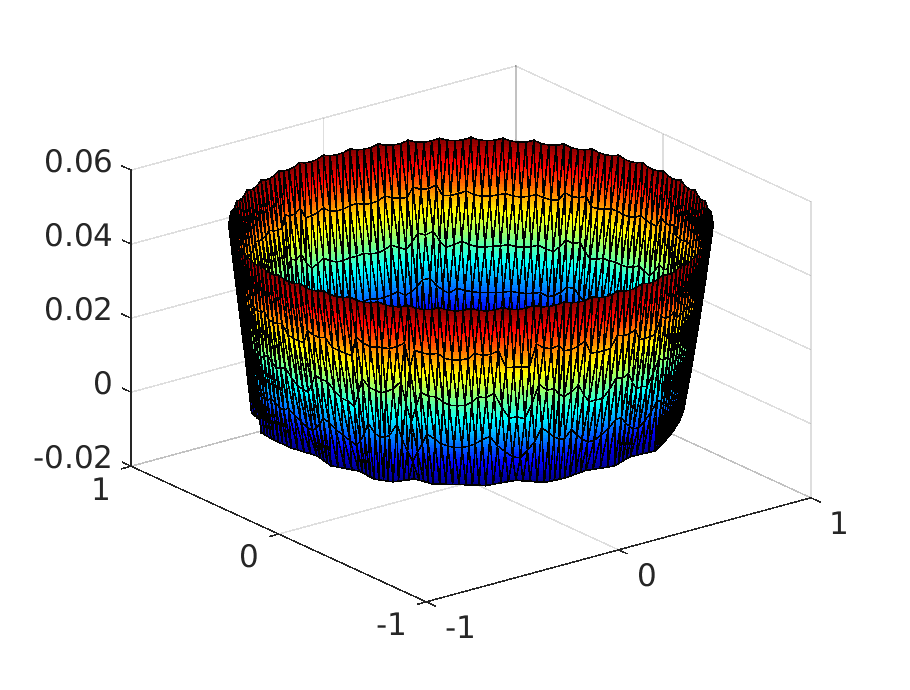
\includegraphics[width=\textwidth]{fig_article/fig_diff_u1_u2_newton_iter_4.eps}    
\label{ref:position_membrane_inside_iter}
\end{subfigure}
\begin{subfigure}[normal]{0.32\textwidth}
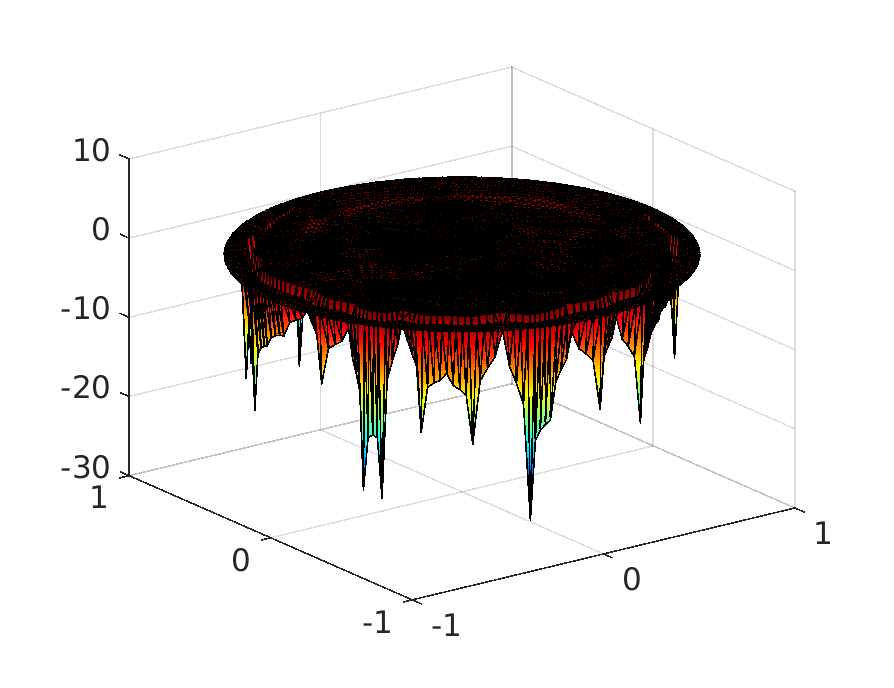
\includegraphics[width=\textwidth]{fig_article/fig_lambda_newton_iter_4.eps}     
\label{ref:lambda_membrane_inside_iter} 
\end{subfigure}
%\caption{membranes (left) and lagrange multiplier (right) during the iterations }
\end{figure}
\vspace{-0.2 cm}
\textcolor{cadmiumgreen}{\textbf{Motivation:}}   $\Ktildeghp = \left\{(\vunh,\vdeuxh) \in \Xghp \times \Xzerohp, \ \vunh-\vdeuxh \geq 0  \right\} \textcolor{red}{\subset \Kg}$.\\ Define $\shki \in \Ktildeghone= \Kghone$ by
\vspace{0.2 cm}
$\dps \shki (\ba)= \dps \begin{cases}
\uhki(\ba) = \left(\uunhki(\ba), \udeuxhki(\ba)\right) \ &\mbox{if $\uunhki(\ba) \geq \udeuxhki(\ba)$,}\\
\dps  \left(1/2 (\uunhki(\ba) + \udeuxhki(\ba)), 1/2 (\uunhki(\ba) + \udeuxhki(\ba))\right) \ &\mbox{if $\uunhki(\ba) < \udeuxhki(\ba)$.}\end{cases}$
\end{frame}
\begin{frame}


\textcolor{cadmiumgreen}{\textbf{Discretization error estimators}}
$\left.
\begin{array}{ll}
\dps {\eta}_{\mathrm{F},K,\ialf}^{\textcolor{royalblue}{k},\textcolor{burntorange}{i}} &= \left\| \mu_\ialf^{\frac{1}{2}} \nab u_{\ialf h}^{\textcolor{royalblue}{k},\textcolor{burntorange}{i}}+\mu_\ialf^{-\frac{1}{2}} \sigialfhdiscki \right\|_{K}  
\\
\dps {\eta}_{\mathrm{osc},K,\ialf} & =  \dps \frac{h_K}{\pi} \mu_\ialf^{-\frac{1}{2}} \left\|f_\ialf-{\bm \Pi}_{\mathbb{P}_1}(f_\ialf)\right\|_{K}\\
\dps \etCKkipos & = 2 \dps \left(\uunhki-\udeuxhki,\lambhkipos\right)_K
\end{array}
\right\} \Rightarrow \dps \textcolor{bulgarianrose}{\bm\eta^{\textcolor{royalblue}{k},\textcolor{burntorange}{i}}_{\mathrm{disc}}}
$\\
\textcolor{cadmiumgreen}{\textbf{Linearization error estimators}}
%%%%%%%%%%
$\left.
\begin{array}{ll}
\dps \etalinunKki  &=  \tnorm{\shki-\uhki}_K  
\\
\dps \etalindeuxKki &= 2 h_{\Omega} \CPF \left(\frac{1}{\mu_1} + \frac{1}{\mu_2} \right)^{\frac{1}{2}} \left\|\lambhkipos\right\|_{\Omega} \tnorm{\shki-\uhki}_K\\
\dps \etalintroisKki &= h_{\Omega} \CPF \left(\frac{1}{\mu_1} + \frac{1}{\mu_2} \right)^{\frac{1}{2}} \left\| \lambhkineg\right\|_K
\end{array}
\right\} \Rightarrow \dps \textcolor{bulgarianrose}{\bm\eta^{\textcolor{royalblue}{k},\textcolor{burntorange}{i}}_{\mathrm{lin}}}
$
\\
\textcolor{cadmiumgreen}{\textbf{Algebraic error estimators}}\\
\vspace{0.1 cm}
$\left.
\begin{array}{ll}
\dps \etaalgKialfki &= \left\|\mu_\ialf^{-\frac{1}{2}}\sigialfhalgki\right\|_{K}
\end{array}
\right\} \Rightarrow \dps \textcolor{bulgarianrose}{\bm\eta^{\textcolor{royalblue}{k},\textcolor{burntorange}{i}}_{\mathrm{alg}}}
$

\begin{theorem}[A posteriori  estimate distinguishing the error components]


\emph{
\textcolor{bulgarianrose}{
\begin{equation*}
\dps
|||\bu-\uhki||| \leq \bm \eta^{\textcolor{royalblue}{k},\textcolor{burntorange}{i}}_{\mathrm{disc}} + \bm \eta^{\textcolor{royalblue}{k},\textcolor{burntorange}{i}}_{\mathrm{alg}} + \bm \eta^{\textcolor{royalblue}{k},\textcolor{burntorange}{i}}_{\mathrm{lin}}.
\end{equation*}
}}

\end{theorem}
\end{frame}

% \begin{frame}
% \vspace{-0.2 cm}
% \begin{proof}
% We define global versions of these estimators as $ \eta_{\cdot}^{k,i} = \left\{\sum_{K \in \Th}\left(\eta_{\cdot,K}^{k,i}\right)^2\right\}^{\frac{1}{2}}$
% \begin{enumerate}
% \item $\uhki \notin \Kgh$: define the projection 
% $\bs$ of $\uhki$ in $\Kg$ by $a(\bs,\bv-\bs) \geq a(\uhki,\bv-\bs) \quad \forall \bv \in \Kg $ \alert{Pb well posed: Lions-Stampacchia}


% \item<2-> 

% $
% \tnorm{\bu-\uhki}^2 = \underbrace{ a(\bu - \uhki, \bu - \bs)}_{=\textcolor{blue}{\textbf{A}}} + \underbrace{a(\bu  - \uhki, \bs-\uhki)}_{=\textcolor{cadmiumgreen}{\textbf{B}}}.
% %=a(\bu,\bu-\uhki)-a(\uhki,\bu-\uhki).
% $
% \item<3-> 

% $\textcolor{cadmiumgreen}{\textbf{B}} \leq \tnorm{\bu-\uhki} \etalinunki$
% \item<4-> 
% \footnotesize
% \vspace{-0.3 cm}
% $\dps
% \textcolor{blue}{\textbf{A}} \leq \left(\underbrace{\left\{\dps \sum_{K \in \Th}\dps \sum_{\ialf=1}^2({\eta}_{\mathrm{osc},K,\ialf} + {\eta}_{\mathrm{F},K,\ialf}^{\textcolor{royalblue}{k},\textcolor{burntorange}{i}})^2\right\}^{\frac{1}{2}}}_{\textcolor{bulgarianrose}{\eta_1}} + \etalintroiski \right) \tnorm{\bu-\uhki} + \frac{1}{2} \etalindeuxki + \frac{1}{2} \sum_{K \in \Th} \etCKkipos 
% $
% \item<5-> 
% \alert{Young inequality:} $\dps \tnorm{\bu-\uhki} \leq  \left\{ \left(\eta_1^{\textcolor{royalblue}{k},\textcolor{burntorange}{i}} + \etalinunki + \etalintroiski    \right)^2  + \etalindeuxki + \sum_K \etCKkipos \right\}^{\frac{1}{2}}.
% $
% \end{enumerate}
% \end{proof}
% \end{frame}

\begin{frame}
\vspace{-0.3 cm}
\begin{algorithm}[H]
\frametitle{Adaptive inexacte semismooth Newton algorithm}
\caption{Adaptive inexact semismooth Newton algorithm}
\begin{algorithmic}

\STATE{\textbf{Initialization:}\; Choose an initial vector $\Xh^{\textcolor{royalblue}{0}} \in \mathcal{M}_{3N_h,1}(\R)$, ($\textcolor{royalblue}{k}=0$)}\\
\STATE{\textbf{Do}}\\
\STATE{\quad$\textcolor{royalblue}{k} =\textcolor{royalblue}{k+1}$}\\
\STATE {\quad Compute $\bbA^{\textcolor{royalblue}{k-1}} \hspace{-0.1
 cm} \in \mathcal{M}_{3N_h,3N_h}(\R)$, $\bB^{\textcolor{royalblue}{k-1}} \hspace{-0.1 cm} \in \mathcal{M}_{3N_h,1}(\R)$ \\
\quad Consider 
%the system of linear algebraic equations 
$\bbA^{\textcolor{royalblue}{k-1}} \Xhk= \bB^{\textcolor{royalblue}{k-1}}$}
\STATE{\quad \textbf{Initialization for the linear solver:} Define $\X_h^{\textcolor{royalblue}{k},\textcolor{burntorange}{0}} = \X_h^{\textcolor{royalblue}{k-1}}$, ($\textcolor{burntorange}{i=0}$) 
%as initial guess for the linear solver 
}\\
\STATE{\quad \textbf{Do}}
	\STATE{\qquad $\textcolor{burntorange}{i=i+1}$}\\	
	\STATE \qquad Compute Residual: {$\Rhki =\bB^{\textcolor{royalblue}{k-1}}-\bbA^{\textcolor{royalblue}{k-1}} \Xhki$}\\
	\qquad  Compute estimators 
	\STATE{\quad \textbf{While} \fcolorbox{violet}{white}{$\textcolor{bulgarianrose}{\bm \eta^{\textcolor{royalblue}{k},\textcolor{burntorange}{i}}_{\mathrm{alg}}} \geq \gamma_{\mathrm{alg}} \max  \left\{{\textcolor{bulgarianrose}{\eta^{\textcolor{royalblue}{k},\textcolor{burntorange}{i}}_{\mathrm{disc}}}, \textcolor{bulgarianrose}{\eta^{\textcolor{royalblue}{k},\textcolor{burntorange}{i}}_{\mathrm{lin}}}}\right\}$}} 
	

	\STATE{\textbf{While} \fcolorbox{violet}{white}{ $\textcolor{bulgarianrose}{\bm \eta^{\textcolor{royalblue}{k},\textcolor{burntorange}{i}}_{\mathrm{lin}}} \geq \gamma_{\mathrm{lin}} \textcolor{bulgarianrose}{\eta^{\textcolor{royalblue}{k},\textcolor{burntorange}{i}}_{\mathrm{disc}}}$}} 
	\STATE{\textbf{End}}
%	\ELSE \STATE{$\textcolor{royalblue}{k}=\textcolor{royalblue}{k}+1$} 

\end{algorithmic}
\end{algorithm}
\end{frame}




\begin{frame}
\section{Numerical experiments}
\subsection{}

\frametitle{Numerical experiments}

\begin{itemize}
\item
$\Omega$ = \mbox{unit disk}, $J = 3$, $\mu_1= \mu_2 = 1$, $g = 0.05$, $\gamma_{\mathrm{lin}}=0.3$ $\gamma_{\mathrm{alg}}=0.3$
\item 
semismooth solver: \textcolor{blue}{Newton-min}. Linear solver: \textcolor{red}{GMRES}
\end{itemize}


\begin{figure}
\begin{minipage}[c]{.34\linewidth}
   \centering
   \quad Exact Newton
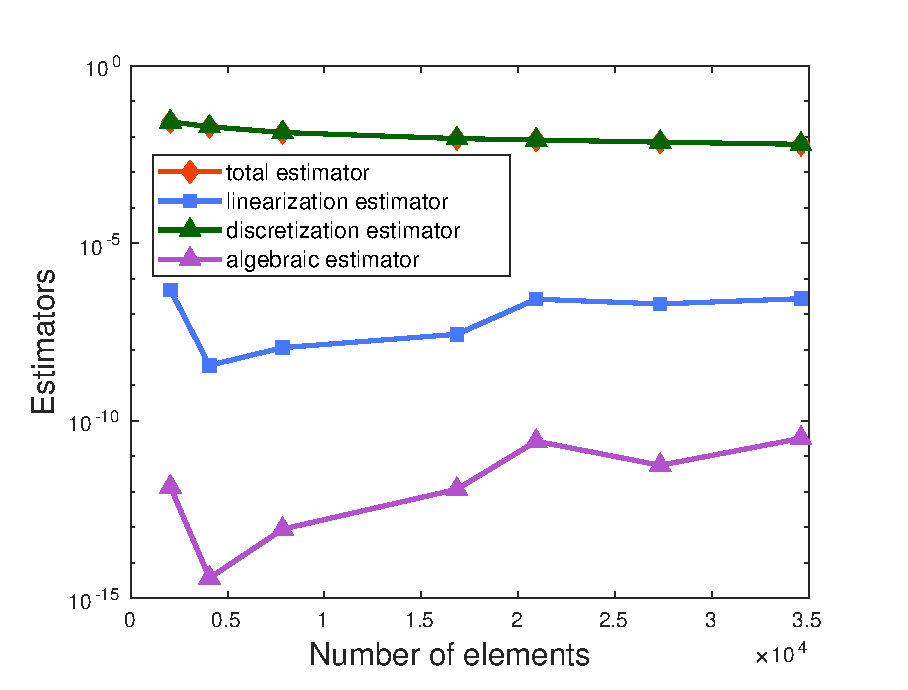
\includegraphics[width=\textwidth]{fig_article/exact_resolution_convergence_estimator_number_elements.eps}    
%\label{ref:position_membrane_convergence}
\end{minipage}\hfill
\begin{minipage}[c]{.33\linewidth}
   \centering
   \quad Inexact Newton
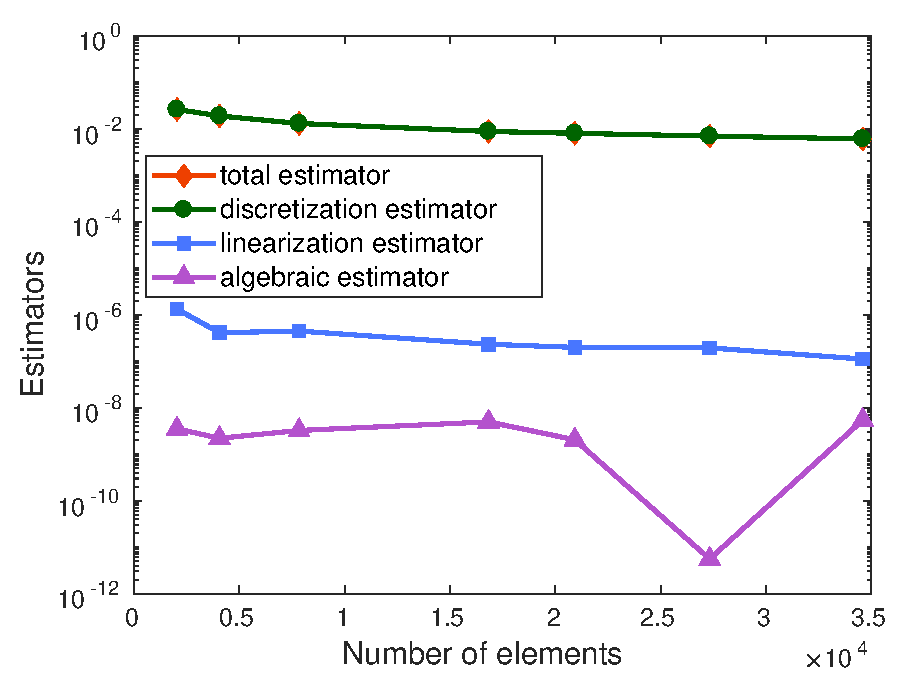
\includegraphics[width=\textwidth]{fig_article/inexact_resolution_convergence_estimator_number_elements.eps}    
%\label{ref:position_membrane_convergence}
\end{minipage}\hfill
\begin{minipage}[c]{.33\linewidth}
   \centering
   Adaptive inexact Newton
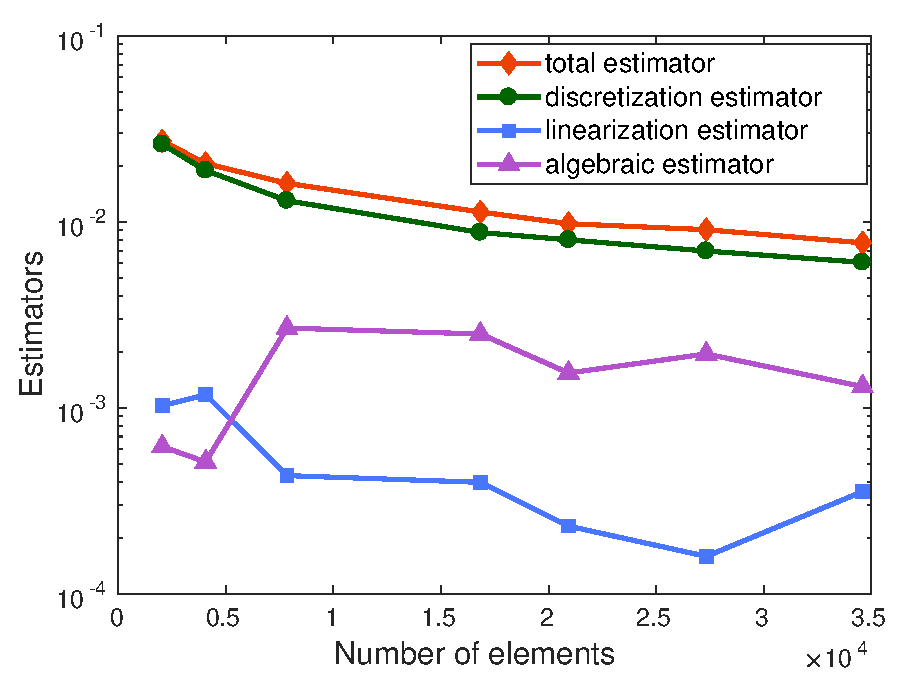
\includegraphics[width=\textwidth]{fig_article/adapt_inexact_resolution_convergence_estimator_number_elements.eps}     
%\label{ref:lambda_membrane_convergence} 
\end{minipage}
%\caption{Exact Newton(left), Inexact Newton(middle), adaptive inexact Newton(right)}
\end{figure}

\textcolor{red}{\textbf{Quality and precision are preserved for adaptive inexact semismooth Newton method.}}


\end{frame}

\begin{frame}
\begin{figure}
\begin{minipage}[c]{.33\linewidth}
   \centering
   Exact Newton
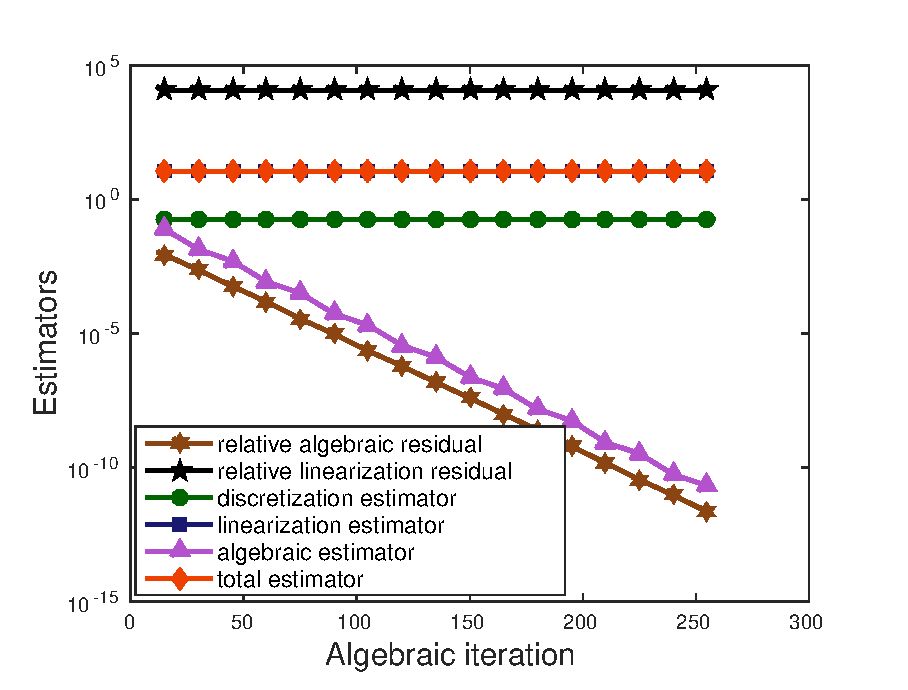
\includegraphics[width=\textwidth]{fig_article/exact_resolution_estimators_gmres_iter_inside_first_newton_iter_Hmax_015.eps}    
%\label{ref:position_membrane_convergence}
\end{minipage}\hfill
\begin{minipage}[c]{.34\linewidth}
   \centering
   Inexact Newton
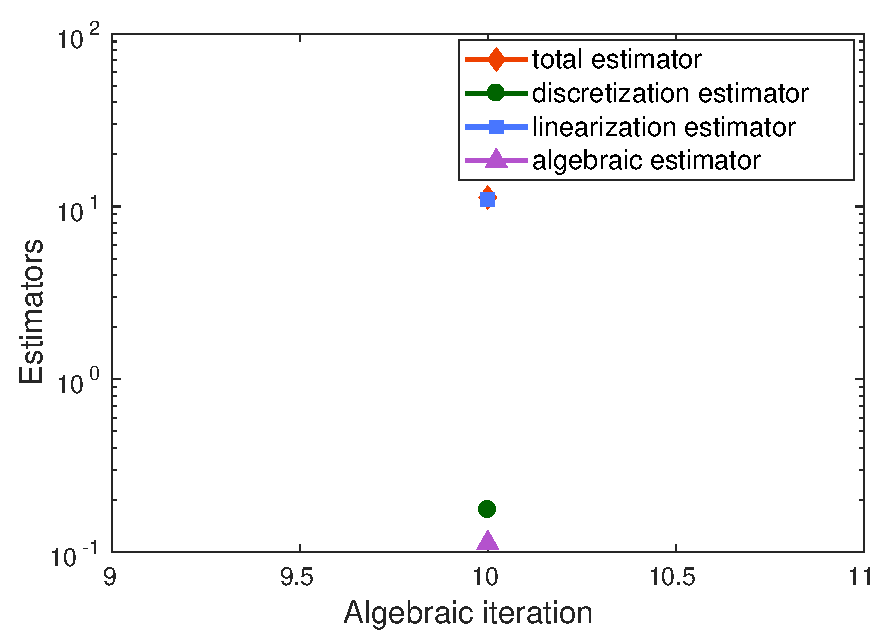
\includegraphics[width=\textwidth]{fig_article/inexacte_resolution_Hmax_015_number_gmres_iter_inside_first_newton_step.eps}    
%\label{ref:position_membrane_convergence}
\end{minipage}\hfill
\begin{minipage}[c]{.33\linewidth}
   \centering
   Adaptive inexact Newton
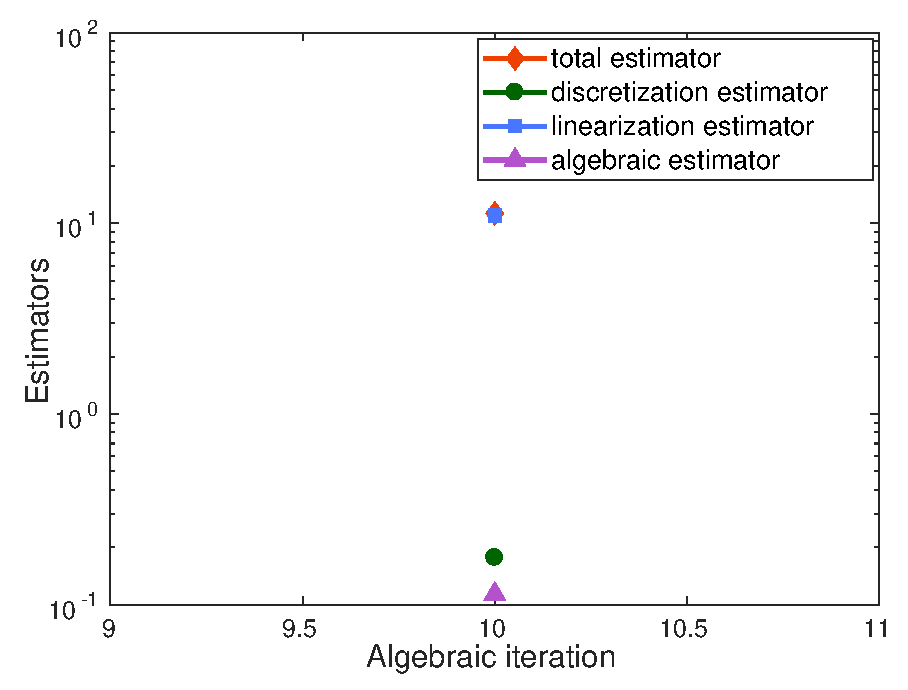
\includegraphics[width=\textwidth]{fig_article/adapt_inexact_resolution_estimators_gmres_iter_inside_first_newton_iter_Hmax_015.eps}     
%\label{ref:lambda_membrane_convergence} 
\end{minipage}
%\caption{Exact Newton(left), Inexact Newton(middle), adaptive inexact Newton(right)}
\end{figure}

\vspace{-0.3 cm}
\begin{figure}
   \begin{minipage}[c]{.33\linewidth}
   \centering
   Exact  Newton 
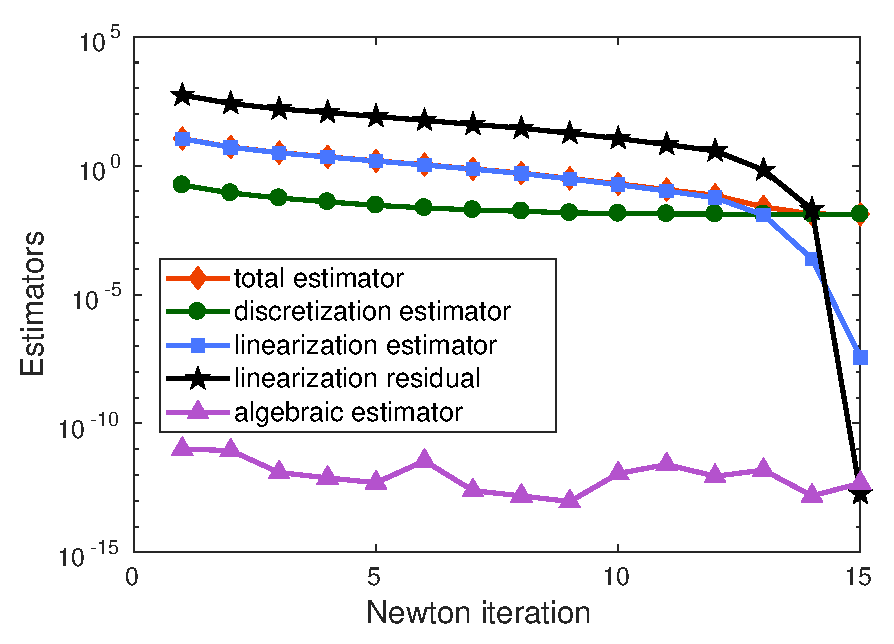
\includegraphics[width=\textwidth]{fig_article/exact_resolution_estimators_newton_iter_Hmax_015.eps}    
   \end{minipage} \hfill
   \begin{minipage}[c]{.33\linewidth}
   \centering
   Inexact Newton
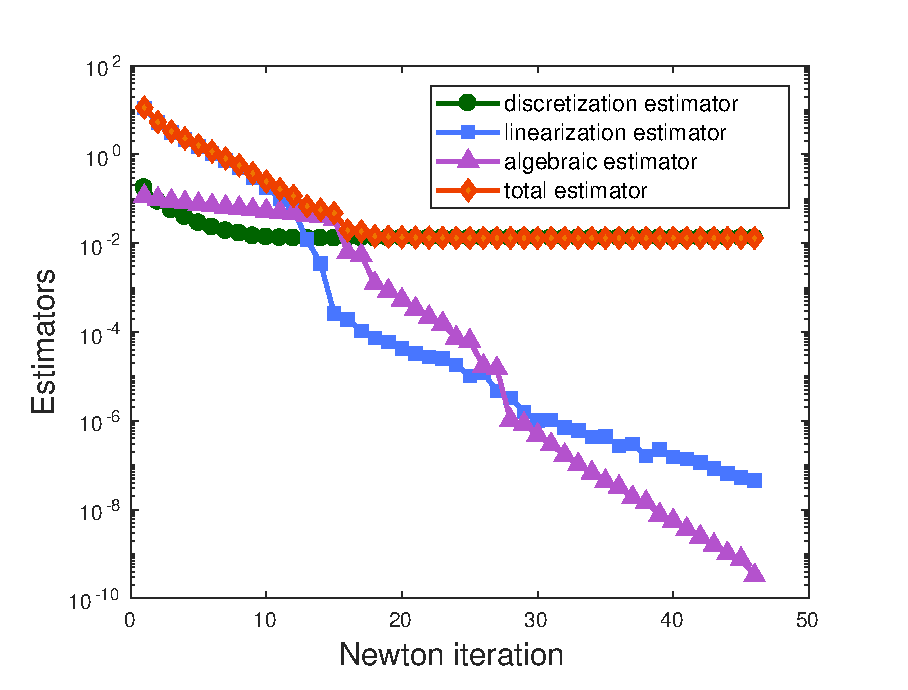
\includegraphics[width=\textwidth]{fig_article/inexacte_resolution_Hmax_015_estimators_newton_step.eps}     
   \end{minipage} \hfill
  \begin{minipage}[c]{.32\linewidth}
  \centering
  Adaptive Inexact Newton  
   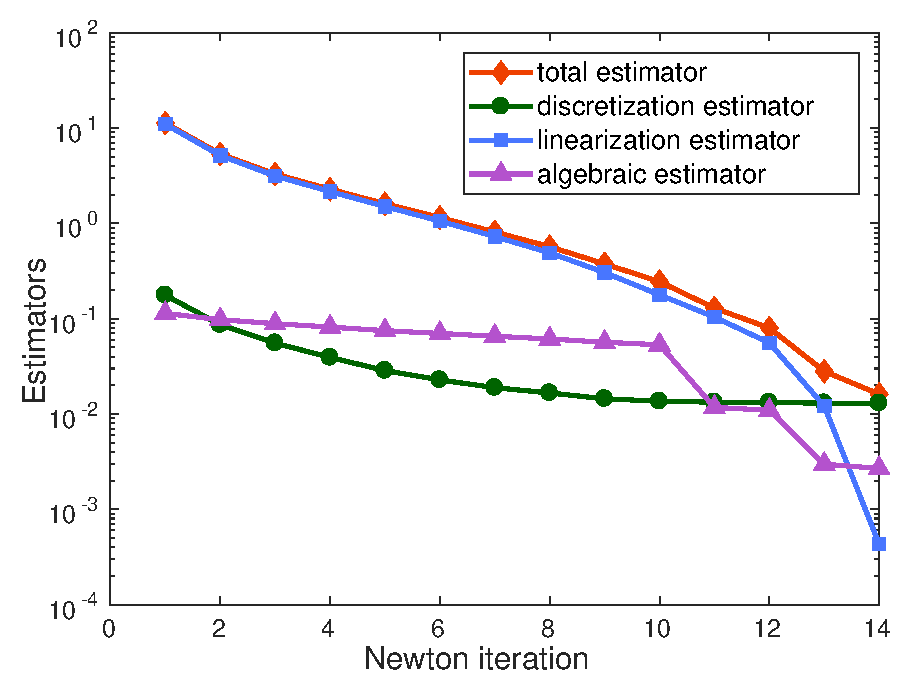
\includegraphics[width=\textwidth]{fig_article/adapt_inexact_resolution_estimators_newton_iter_Hmax_015.eps}     
\end{minipage}\hfill
\end{figure}
\end{frame}

\begin{frame}

\textcolor{red}{\textbf{Overall performance of the three approaches:}}
\begin{figure}[H]
\begin{minipage}[c]{.42\linewidth}
   \centering 
   Newton
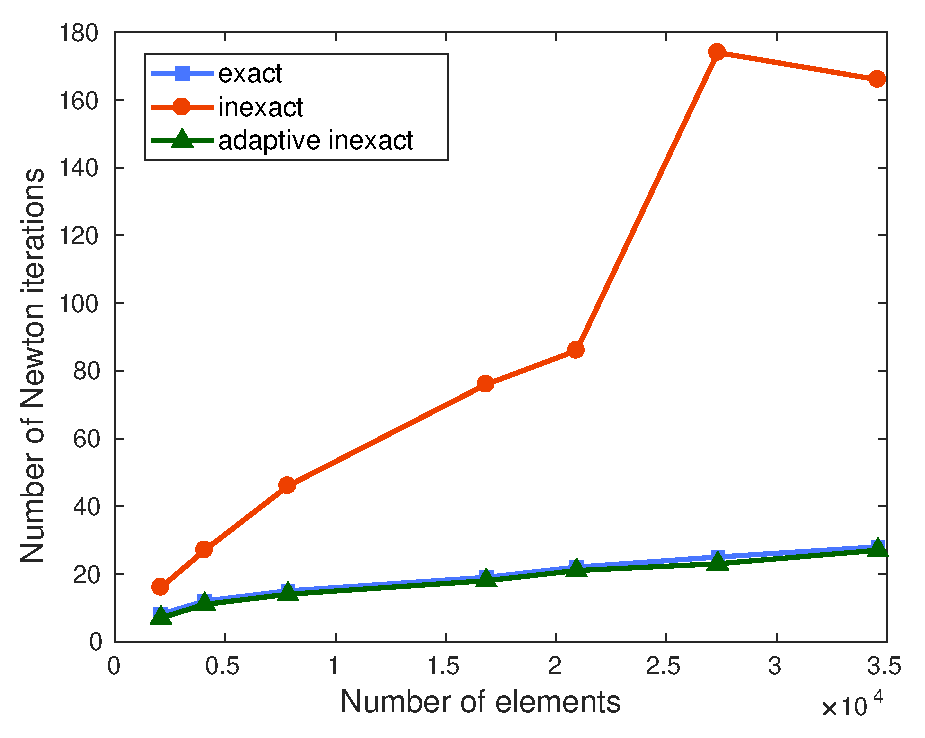
\includegraphics[width=\textwidth]{fig_article/comparison_three_methods_number_Newton_iter_number_elements.eps}    
%\label{ref:position_membrane_convergence}
\end{minipage}\hfill
\begin{minipage}[c]{.44\linewidth}
\centering
GMRES
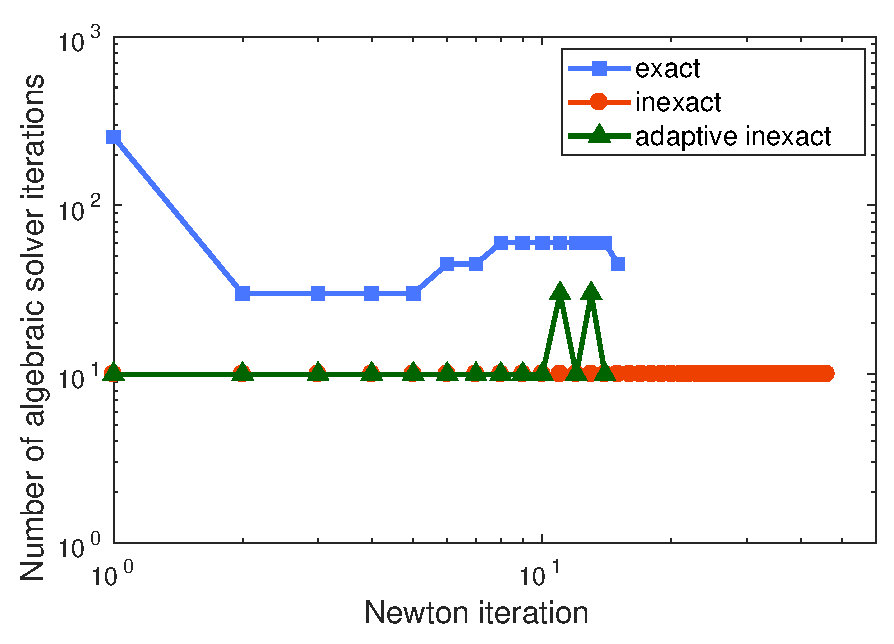
\includegraphics[width=\textwidth]{fig_article/comparison_three_methods_number_Gmres_iter_number_newton_step.eps}    
%\label{ref:position_membrane_convergence}
\end{minipage} \hfill
\end{figure}
\begin{figure}
\vspace*{-0.04\textwidth} \hspace*{0.1\textwidth}
\begin{minipage}{.41\linewidth} 
\centering   Total GMRES
 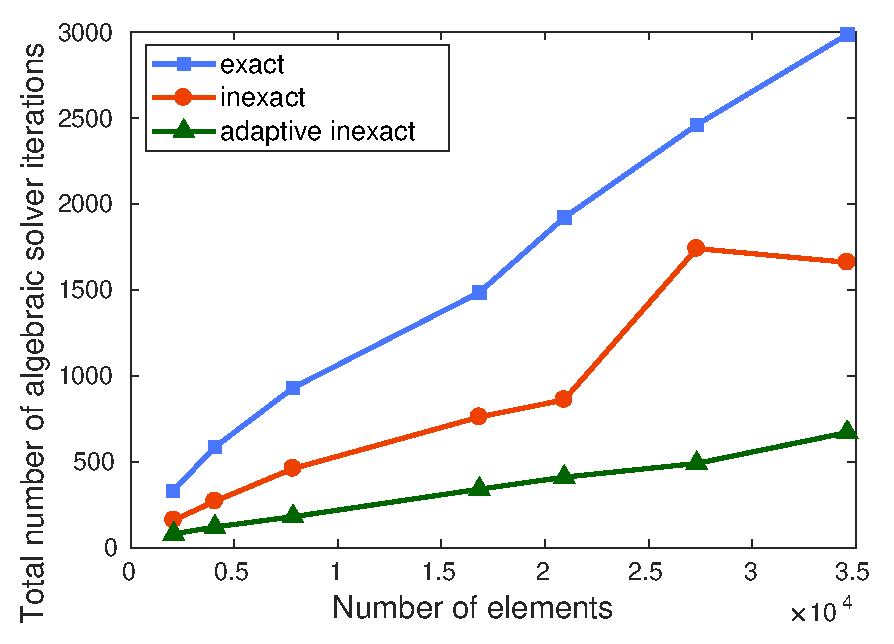
\includegraphics[width=\textwidth]{fig_article/comparison_three_methods_total_number_Newton_Gmres_iter_number_elements.eps}     
%\label{ref:lambda_membrane_convergence} 
\end{minipage} \hfill

%\caption{Number of Newton iterations per number of elements (left), number of linear solver iterations per Newton step, and total number of linear solver iterations per number of elements}
\label{ref:figure:plot:number:alg:iter:per:newton:step}
\end{figure}
\end{frame}
%\begin{frame}
%%\begin{figure}[H]
%\centering
%\begin{tabular}
%{|>{\begin{bf}} c <{\end{bf}}|c|c|c|c|c|}
%\hline
% $(\gamma_{\mathrm{alg}},\gamma_{\mathrm{lin}})$  & 
% $(0.1,0.1)$ &  $(0.01,0.1)$  & $(0.1,0.01)$ & $(0.01,0.01)$ \\
%\hline
% Newton iter &   21 &  21 &  25 &  25  \\
%\hline
% Algebraic  iter ($k=5$) &   10 &  30 &  10 &  30\\
%\hline
% Total iter &   210 &  370 &  250 &  410 
%\label{ref:tableau:number:inex:adapt:iter_gamma:alg:0.1}
%%\caption{Adaptive inexact Newton method for a fixed mesh containing approximately 35000 elements and for several weights $\gamma_{\mathrm{alg}}$ and $\gamma_{\mathrm{lin}}$.}
%\label{ref:tableau:comparatif}
%
%\end{tabular}
%%\end{figure}
%\end{frame}

\begin{frame}
\begin{figure}
\begin{minipage}[c]{.46\linewidth}
   \centering
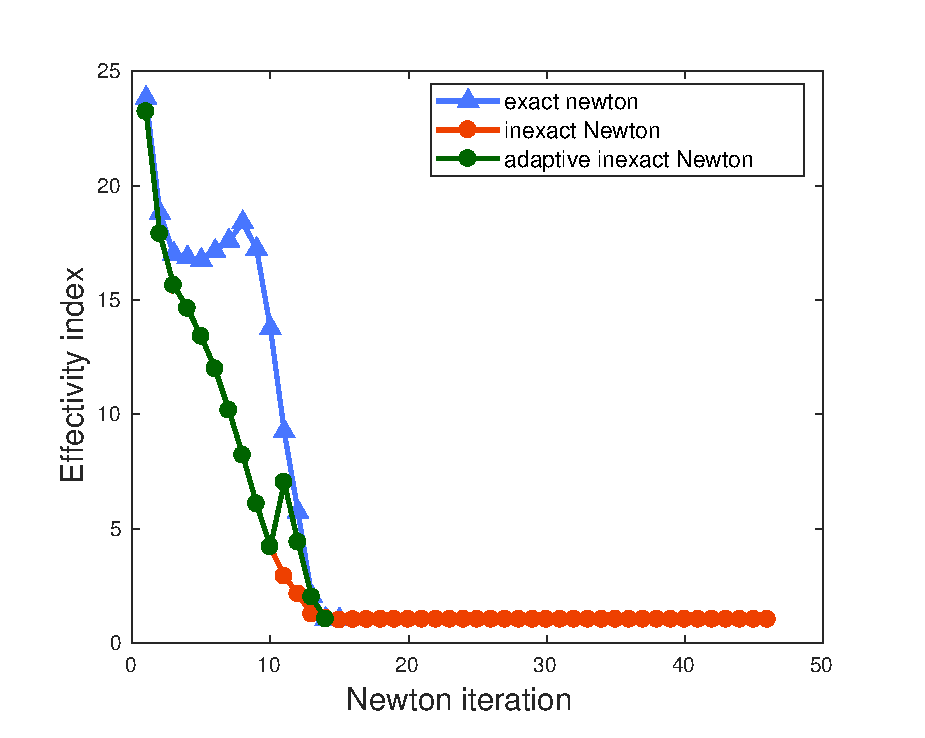
\includegraphics[width=\textwidth]{fig_article/effectivity_index_3_methods_Hmax_015.eps}    
%\label{ref:position_membrane_convergence}
\end{minipage}\hfill
\begin{minipage}[c]{.46\linewidth}
   \centering
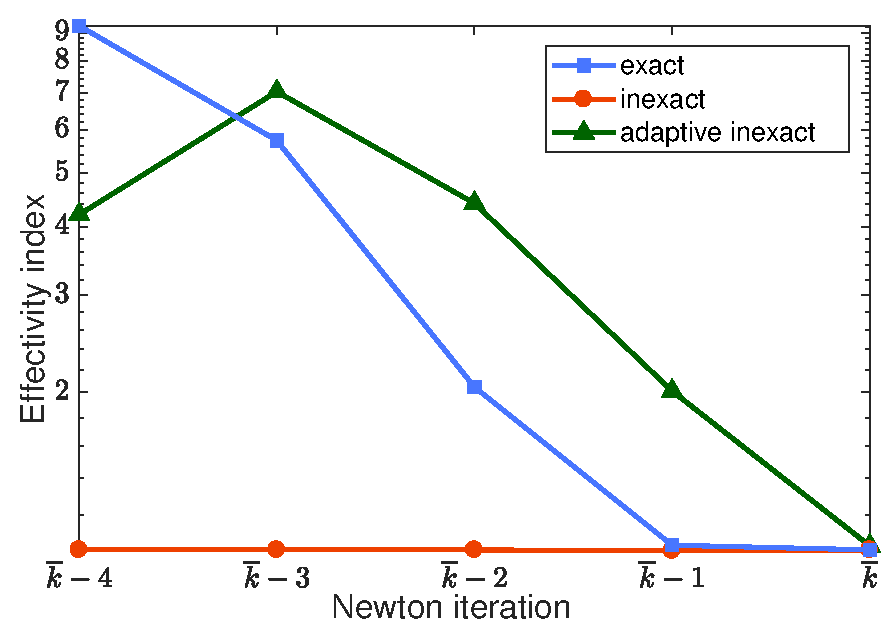
\includegraphics[width=\textwidth]{fig_article/effectivity_index_3_methods_last_newton_iter_Hmax_015.eps}     
%\label{ref:lambda_membrane_convergence} 
\end{minipage}\hfill
\begin{minipage}[c]{.48\linewidth}
   \centering
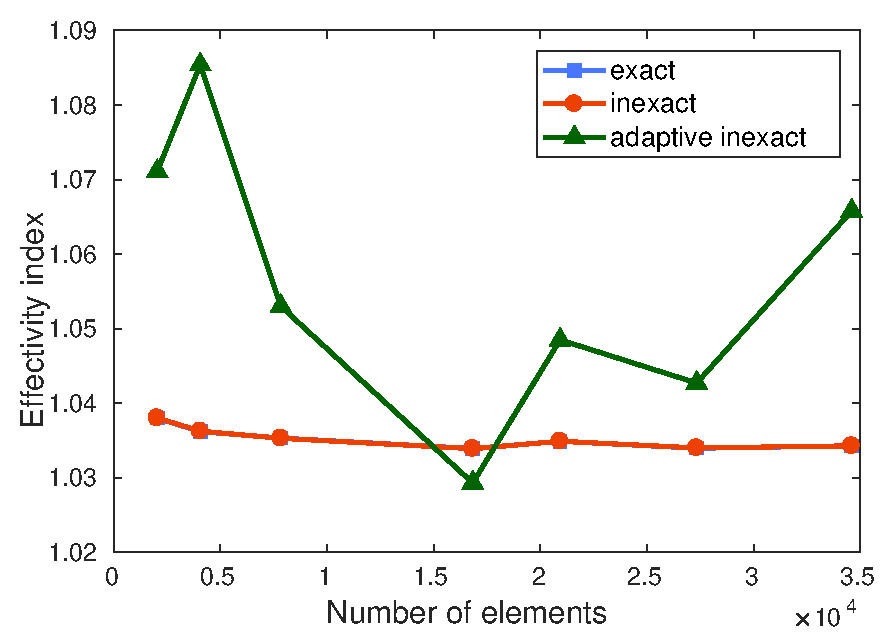
\includegraphics[width=\textwidth]{fig_article/effectivity_index_3_methods_number_elements.eps}     
%\label{ref:lambda_membrane_convergence} 
\end{minipage}
\end{figure}
\end{frame}
\begin{frame}
\center\textcolor{red}{\textbf{\LARGE Distribution of the error:}}
\vspace*{1 cm}
\begin{figure}[H]
\begin{minipage}[c]{.5\linewidth}
   \centering
   Actual error
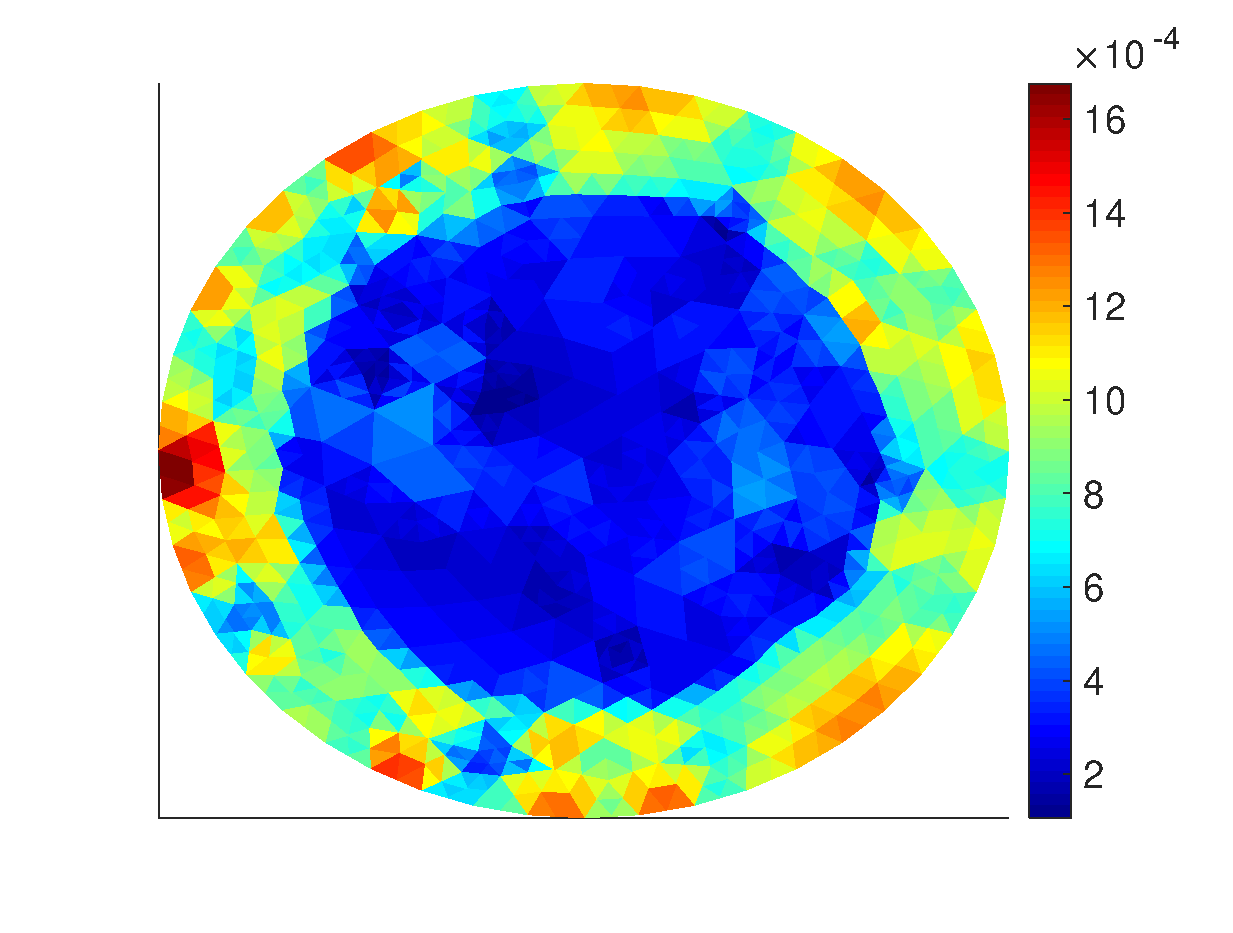
\includegraphics[width=\textwidth]{fig_article/estimator_actual_error_inexact_newton_iter_30second_level.eps}    
%\label{ref:position_membrane_convergence}
\end{minipage}\hfill
\begin{minipage}[c]{.5\linewidth}
   \centering
   Estimated error
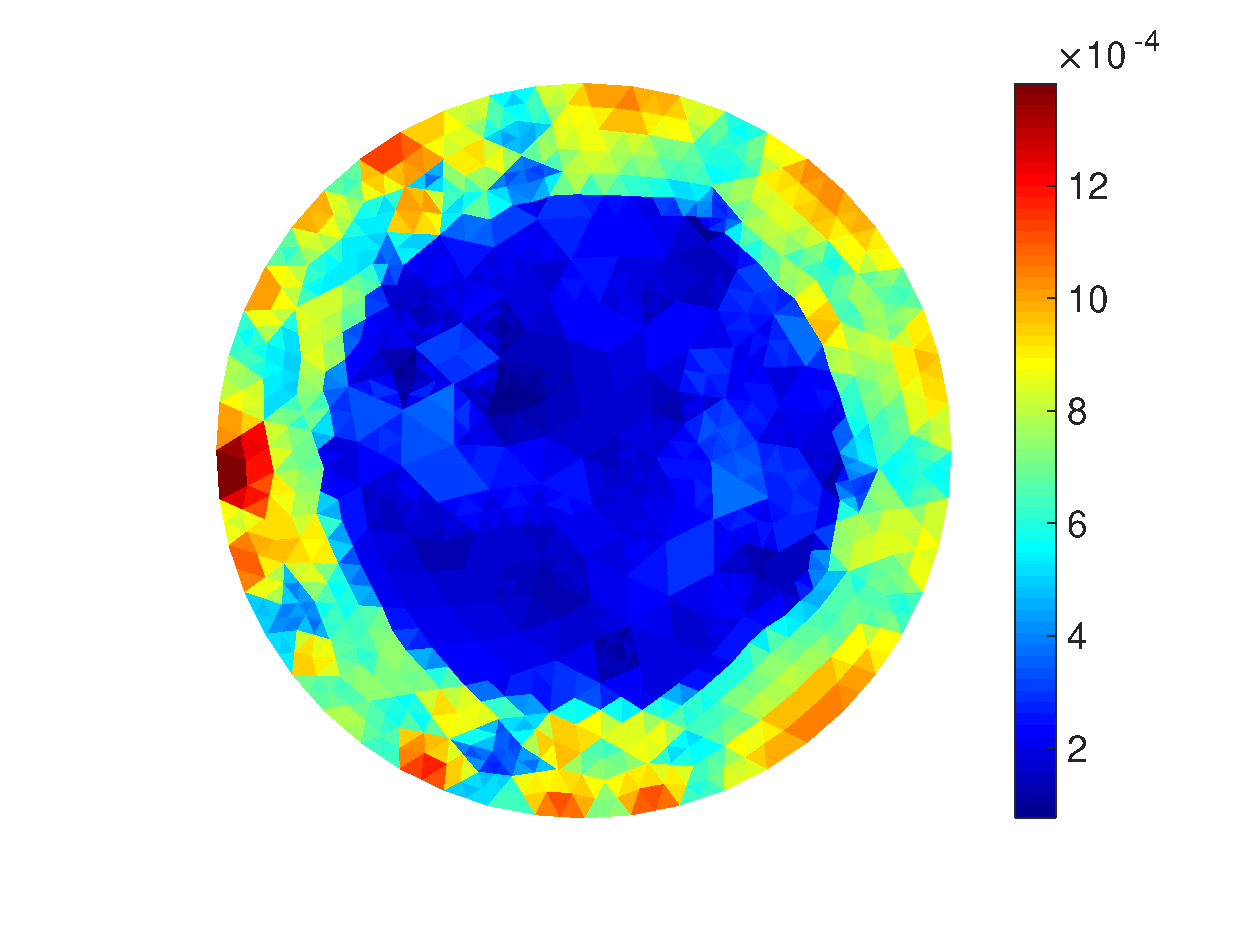
\includegraphics[width=\textwidth]{fig_article/energy_norm_second_level_inexact_newton_iter_30.eps}     
%\label{ref:lambda_membrane_convergence} 
\end{minipage}\hfill
%\caption{Estimated(left) and actual(right), $J=2$, inexact Newton}
\end{figure}

\end{frame}
\begin{frame}
\frametitle{Conclusion}
\begin{itemize}
\item
We devised an a posteriori error estimate between $\bu$ and $\uhki$ for a wide class of semismooth Newton methods.
\vspace{0.5 cm}

\item 
This estimate enables to control the error at each semismooth Newton step.
\vspace{0.5 cm}
\item
The adaptive inexact semismooth Newton method requires less nonlinear and linear steps.
\vspace{0.5 cm}
\item
Ongoing work: extension to unsteady problems with nonlinear complementarity constraints
\vspace{0.3 cm}
\end{itemize}
\begin{thebibliography}{10}
\scriptsize{
\bibitem{Dabaghi:2017}
{\sc J.~Dabaghi, V.~Martin, and M.~Vohral{\'{\i}}k}, {\em Adaptive inexact
  semismooth Newton methods for the contact problem between two membranes}.
\textcolor{black}{submitted for publication.}
}
\end{thebibliography}

\begin{thebibliography}{10}
\scriptsize{
\bibitem{Dabaghi:2018}
{\sc I.~Ben Gharbia, J.~Dabaghi, V.~Martin, and M.~Vohral{\'{\i}}k}, {\em A posteriori error estimates and adaptive stopping criteria, for a compositional two-phase flow with nonlinear complementarity constraints}.
\textcolor{black}{In preparation, 2018.}
}

\end{thebibliography}

\vspace{1 cm}
\Large
\hspace{1.8 cm}
\textcolor{midnightblue}
{\textbf{
Thank you for your attention!}}
\end{frame}
%\begin{frame}
%\footnotesize
%\frametitle{Bibliography}
%\begin{itemize}
%\item
%Problem of contact between two membranes
%\end{itemize}
%\begin{thebibliography}{10}
%  \bibitem{VorBer:2008}
%Faker Ben~Belgacem, Christine Bernardi, Adel Blouza, and Martin
%  Vohral{\'{\i}}k.
%\newblock A finite element discretization of the contact between two membranes.
%\newblock {\em M2AN Math. Model. Numer. Anal.}, 43(1):33--52, 2008.
%\bibitem{VorBer:2012}
%Faker Ben~Belgacem, Christine Bernardi, Adel Blouza, and Martin
%  Vohral{\'{\i}}k.
%\newblock On the unilateral contact between membranes. {P}art 2: {\it a
%  posteriori} analysis and numerical experiments.
%\newblock {\em IMA J. Numer. Anal.}, 32(3):1147--1172, 2012.
%
%\end{thebibliography}
%\begin{itemize}
%\item
%Inexact Newton method and a posteriori adaptivity
%\end{itemize}
%\begin{thebibliography}{10}
%\bibitem{VorErn:2013}
%Alexandre Ern and Martin Vohral{\'{\i}}k.
%\newblock Adaptive inexact {N}ewton methods with a posteriori stopping criteria
%  for nonlinear diffusion {PDE}s.
%\newblock {\em SIAM J. Sci. Comput.}, 35(4):A1761--A1791, 2013.
%\end{thebibliography}
%
%\begin{itemize}
%\item
%Non smooth analysis and complementarity problem
%\end{itemize}
%\begin{thebibliography}{10}
%
%\bibitem{Facchinei:2003}
%Francisco Facchinei and Jong-Shi Pang.
%\newblock {\em Finite-dimensional variational inequalities and complementarity
%  problems. {V}ol. {I,II}}.
%\newblock Springer Series in Operations Research. Springer-Verlag, New York,
%  2003.
%
%%\bibitem{Pang:2003}
%%Francisco Facchinei and Jong-Shi Pang.
%%\newblock {\em Finite-dimensional variational inequalities and complementarity
%%  problems. {V}ol. {II}}.
%%\newblock Springer Series in Operations Research. Springer-Verlag, New York,
%%  2003.
%  \end{thebibliography}

%\end{frame}

%\begin{frame}
%\begin{center}
%{\Large \textbf {Thank you for your attention}}
%\end{center}
%\end{frame}
\bibliographystyle{plain}
\bibliography{biblio}
\end{document}
